\chapter{Selection of Receiver Architecture}
\label{chap:rx}

A wide variety of different receiver designs exists each with it's advantages
and drawbacks. To come up with an optimal design, different receiver designs
were investigated using theoretical considerations and some were simulated to
further understand them. Thereby the focal point was on architectures we could
build in hardware using the Sivers IMA 58-63 GHz converter described in
\secref{sec:comp_sives}. \\

The following secions cover three different architectures. There are example
frequencies given that are supported by the hardware available. Also their
advantages and drawbacks are disscussed.

\section{Transmitter Architecture}
During this report always the same transmitter architecture was used.
It consists of two channel \gls{DAC} converting the 1.8 GHz wide
\gls{TX} \gls{IF} signal at $f_{\text{TX IF}}$ and a $90^\circ$ phase shifted
version. \\

This two signals are than up-converter to
\gls{RF} and a $90^\circ$ coupler is used to suppress the \gls{LSBand}
as good as possible.
Therefor the \gls{USBand} considered the desired signal and the
not redidual \gls{LSBand} an interferer. \\

It was measured that in our setup the \gls{TX} \gls{LO} leackage
to the output \gls{RF} signal has similar power than the desired
signal it self. Therefor this leackage has to be considered and is
shown in all of the following spectrum drawing.
$f_{\text{TX IF}} = f_{\text{c}} - f_{\text{TX LO}}$ can be chosen accordingly
such that this leackage can be well enough suppressed.

\section{Receiver Architecture}
\subsection{Quadrature Baseband Sampling Receiver}
\label{sec:rx_0}

The Quadrature Baseband Sampling Receiver drawn in \figref{fig:rx_0_bd}
starts with a band filter which is the same for all three architecurs
(see \figref{fig:rx_0_rf}).
It is used to minimize the total power supplied to a \gls{LNA}
which has the main influence of the total noise figure of the receiver
and limits the maximum bandwidth which is downmixed.
Unfortenutely ajastable \gls{RF} filters are very hard to build. Therefor
the band filter is fixed to the whole band of interest. \\

Then a first mixer uses a \gls{LO} $f_{\text{RX LO}} = 55 \text{GHz}$
to mix the signal at $f_{\text{c}} = 60.9 \text{GHz}$
to an \gls{IF} of $f_{\text{RX IF}} = f_{\text{c}} - f_{\text{RX LO}}$
(see \figref{fig:rx_0_freq_rx_if1}).
The two signals $\pm (f_{\text{c}} + f_{\text{RX LO}})$ are not relevant
since their frequency is above 100 GHz and well beyond what the
mixer output can drive. $f_{\text{RX IF}}$ has to be high enough such
that $-f_{\text{c}} + f_{\text{RX LO}}$ does not convolve with the
desired signal which give a lower bound
$f_{\text{RX IF}} \geq \text{BW}_{\text{band filter}}$ for the \gls{RX}
\gls{IF} frequency\footnote{%
  Infact $f_{\text{RX IF}} \geq \frac{\text{BW}_{\text{band filter}}}{2}$
  is sufficient if later stages of the receiver can switch
  between \gls{USBand} and \gls{LSBand}.}. \\

A fixed channel filter is than used to suppress neighbouring channels
including the \gls{TX} \gls{LO} leackage witch was also mixed down. \\

Since our signal is assymetric the baseband signal is not analytic
and therefor quadrature sampling is used.
Hence two mixers using a \gls{LO} at $f_{\text{LO}_2} = 0.9 \text{GHz}$ are
used to downmix the signal to a quadrature baseband which than can
be sampled by two \glspl{ADC} as shown in \figref{fig:rx_0_freq_rx_if2}. \\

Self-mixing of the \gls{LO} of these mixers lead to a \gls{DC}-offset
which has to be blocked in order for the \glspl{ADC} to work at full range.
Therefor all \glspl{ADC} are always used with \gls{DC}-blocks as described in
\secref{sec:sec:comp_dc_block}. This high-pass filters unfortunately
not only remove \gls{DC} but also a small portion of the signal
resulting in some \gls{ISI}. \\

\begin{figure}[ht]
  \centering
  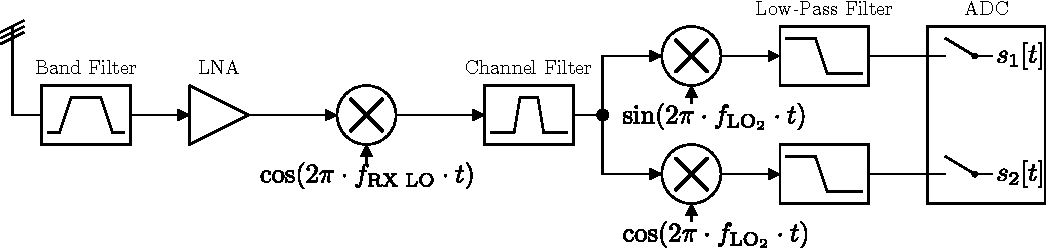
\includegraphics[width=\textwidth]{figures/rx_0_bd}
  \caption{Block Diagram of Quadrature Baseband Sampling Receiver}
  \label{fig:rx_0_bd}
\end{figure}

\begin{figure}[ht]
  \begin{subfigure}{\textwidth}
    \centering
    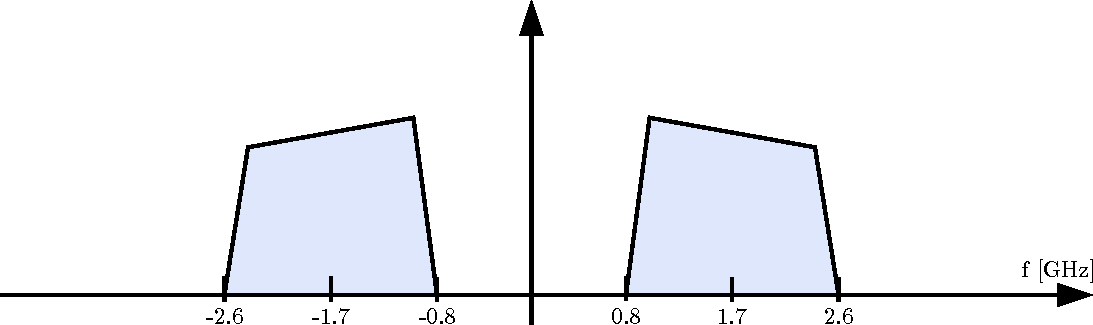
\includegraphics[width=0.8\textwidth]{figures/rx_0_freq_tx_if}
    \caption{\gls{TX} \gls{IF}}
    \label{fig:rx_0_frq_tx_if}
  \end{subfigure}
  \vspace{4ex} \\
  \begin{subfigure}{\textwidth}
    \centering
    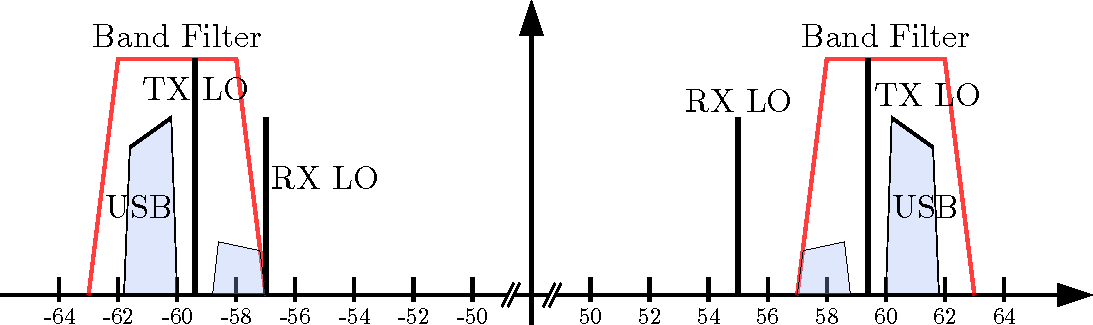
\includegraphics[width=0.8\textwidth]{figures/rx_0_freq_rf}
    \caption{\gls{RF}}
    \label{fig:rx_0_freq_rf}
  \end{subfigure}
  \vspace{4ex} \\
  \begin{subfigure}{\textwidth}
    \centering
    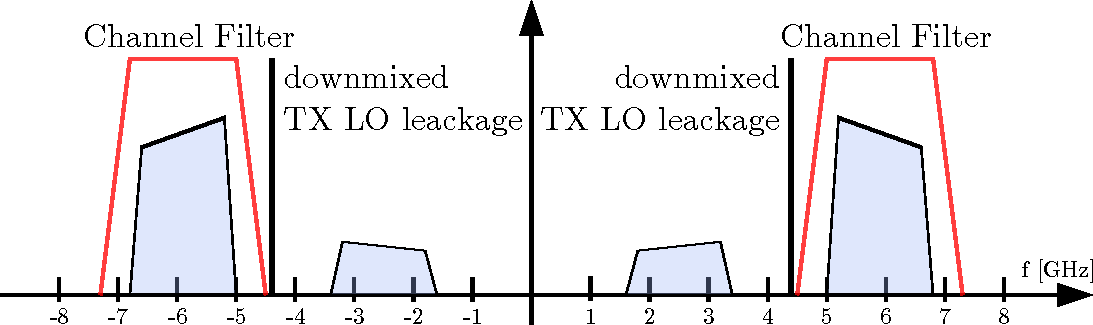
\includegraphics[width=0.8\textwidth]{figures/rx_0_freq_rx_if1}
    \caption{\gls{RX} high \gls{IF}}
    \label{fig:rx_0_freq_rx_if1}
  \end{subfigure}
  \vspace{4ex} \\
  \begin{subfigure}{\textwidth}
    \centering
    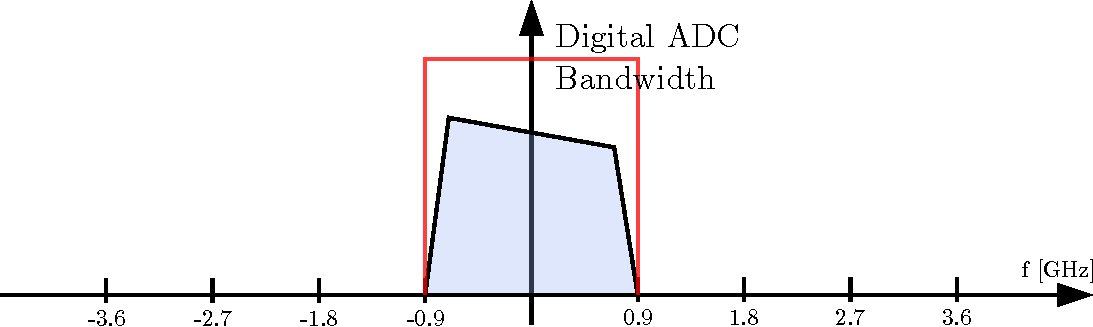
\includegraphics[width=0.8\textwidth]{figures/rx_0_freq_rx_if2}
    \caption{\gls{RX} low \gls{IF}}
    \label{fig:rx_0_freq_rx_if2}
  \end{subfigure}
  \caption{Quadrature Baseband Sampling Receiver in Frequency Domain}
  \label{fig:rx_0_freq}
\end{figure}

\subsection{Intermediate Frequency Sampling Receiver}
\label{sec:rx_1}
\begin{itemize}
\item Two mixer paths and $90^\circ$ couplers can be used to optain a
  single sided donmixed signal
\item High-Pass filter removes signal between RX $\text{LO}_1$ and channel (including TX LO)
\item Second Mixer mixes to first Nyquist zone, Low-Pass filter avoids aliasing
\item RX and TX-LO offset to make sure sent LSB residual does not possitively
  interfer with signal by non perfect LSB suppression in RX.
\item Pro: No high first IF to suppress LSB
\item Con: Sharp high- / low-pass Filter needed
\item Con: high ADC sampling speed
\item Presentation: show theory of 90 deg cancelation
\end{itemize}

A second mixer is than used to mix the desired signal to first Nyquist-zone
of the ADC and sampled at twice the bandwidth
(3.6 GHz for the 1.8 GHz wide signal). Self-mixing of the

\begin{figure}[ht]
  \centering
  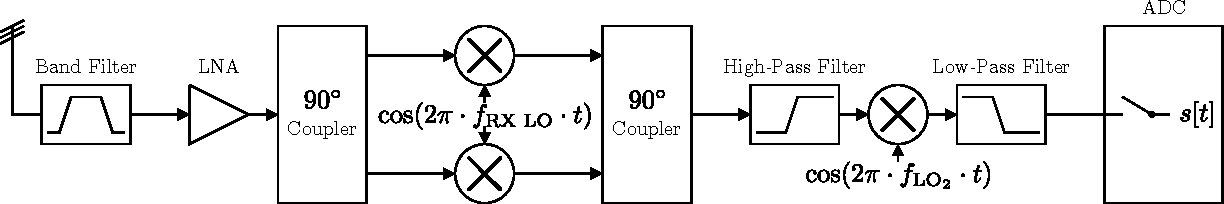
\includegraphics[width=\textwidth]{figures/rx_1_bd}
  \caption{Block Diagram of Intermediate Frequency Sampling Receiver}
  \label{fig:rx_1_bd}
\end{figure}

\begin{figure}[ht]
  \begin{subfigure}{\textwidth}
    \centering
    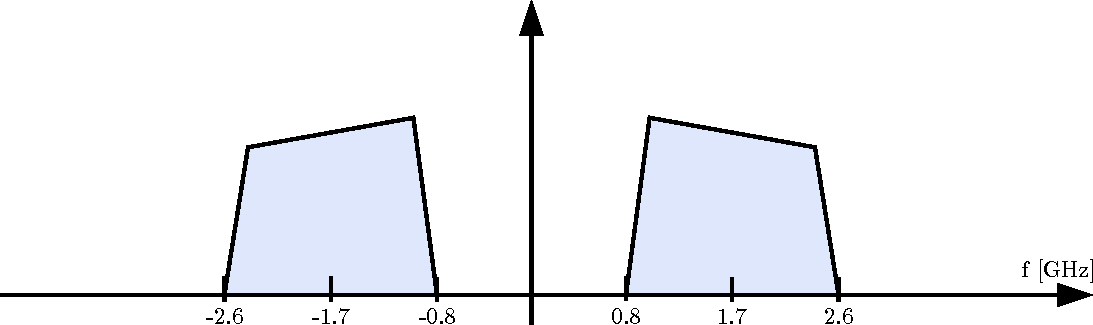
\includegraphics[width=0.8\textwidth]{figures/rx_1_freq_tx_if}
    \caption{\gls{TX} \gls{IF}}
    \label{fig:rx_1_frq_tx_if}
  \end{subfigure}
  \vspace{4ex} \\
  \begin{subfigure}{\textwidth}
    \centering
    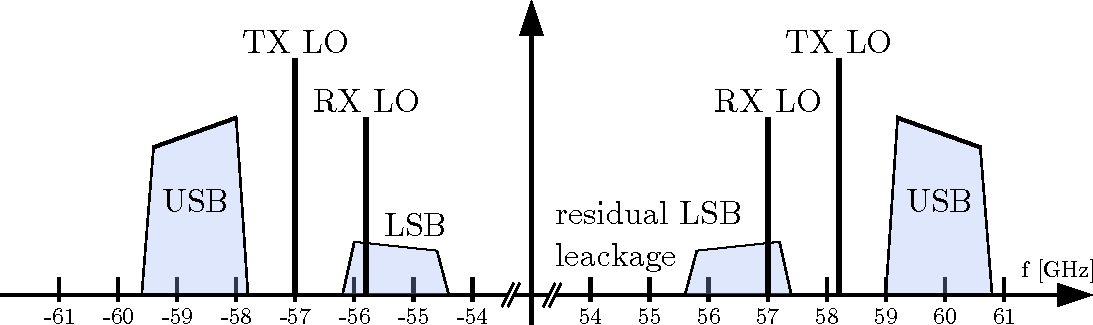
\includegraphics[width=0.8\textwidth]{figures/rx_1_freq_rf}
    \caption{\gls{RF}}
    \label{fig:rx_1_freq_rf}
  \end{subfigure}
  \vspace{4ex} \\
  \begin{subfigure}{\textwidth}
    \centering
    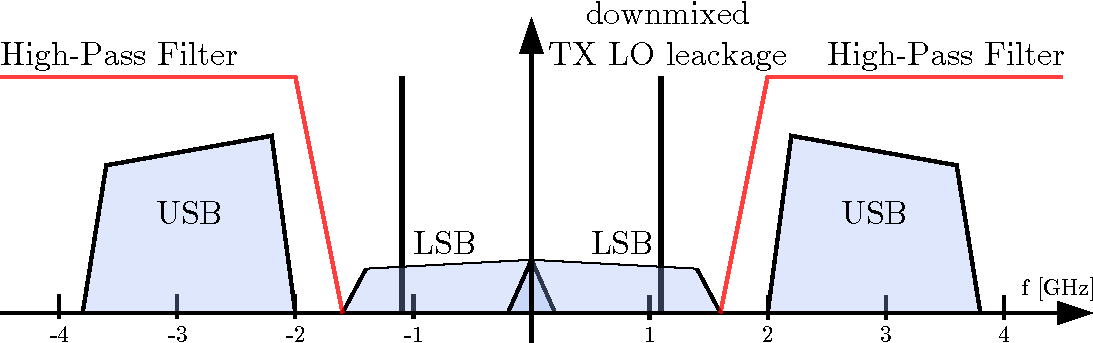
\includegraphics[width=0.8\textwidth]{figures/rx_1_freq_rx_if1}
    \caption{\gls{RX} high \gls{IF}}
    \label{fig:rx_1_freq_rx_if1}
  \end{subfigure}
  \vspace{4ex} \\
  \begin{subfigure}{\textwidth}
    \centering
    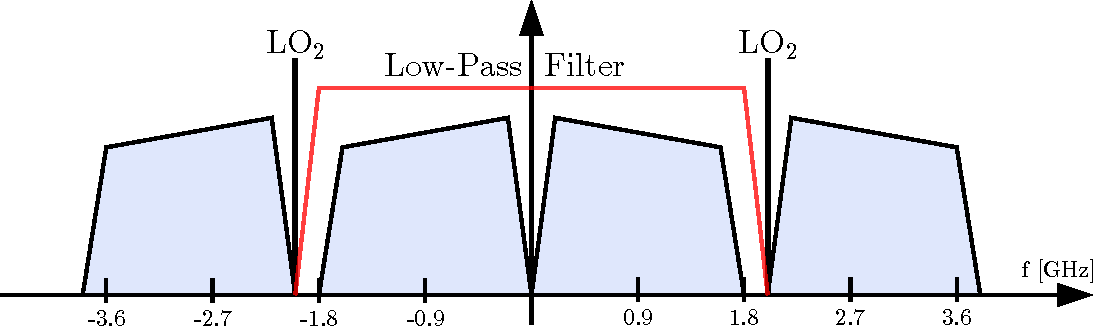
\includegraphics[width=0.8\textwidth]{figures/rx_1_freq_rx_if2}
    \caption{\gls{RX} low \gls{IF}}
    \label{fig:rx_1_freq_rx_if2}
  \end{subfigure}
  \caption{Intermediate Frequency Sampling Receive in Frequency Domain}
  \label{fig:rx_1_freq}
\end{figure}

\subsection{Quadrate Intermediate Frequency Sub-Nyquist Sampling Receiver}
\begin{itemize}
\item USB / LSB problem similar to IF-Mixer image suppression
\item Problem can be solved by using only one mixer and quadrature sampling.
\item Needs double the bandwidth to sample both channels with the full
  signal bandwidth
\item Use sub-nyquist sampling to avoid DC-offset problem and low-frequency
  limitation of components (carrier leakage)
\item Only very few components needed -> less non-idealities
\item since mixer works at much high frequencies than the second mixer of
  previous architectures, much bigger LO-leackage -> cannot work down to DC
\end{itemize}

\begin{figure}[ht]
  \centering
  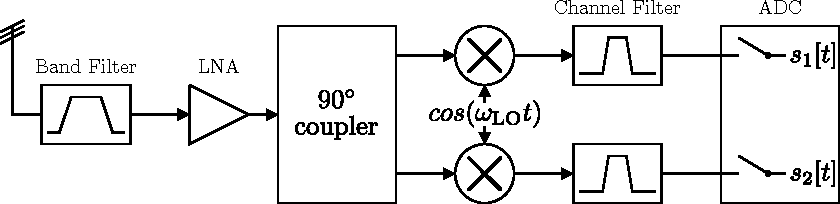
\includegraphics[width=\textwidth]{figures/quad_if_rx_block_diagram}
  \caption{Block Diagram of Quadrate Intermediate Frequency Sub-Nyquist Sampling Receiver}
  \label{fig:rx_2_bd}
\end{figure}

\begin{figure}[ht]
  \begin{subfigure}{\textwidth}
    \centering
    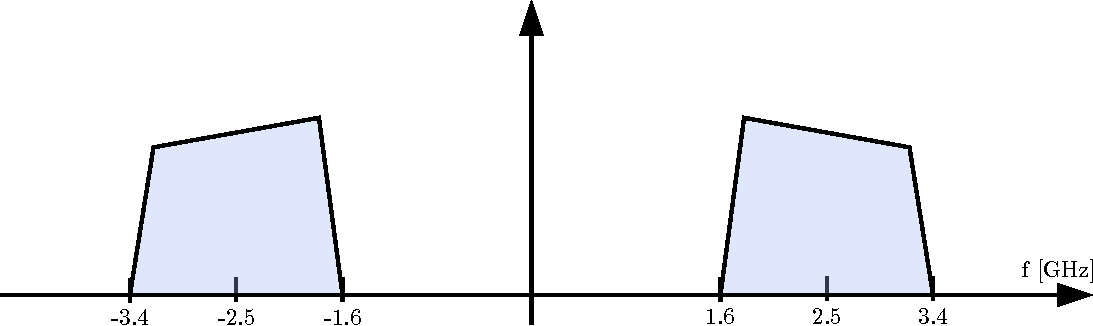
\includegraphics[width=0.8\textwidth]{figures/rx_2_freq_tx_if}
    \caption{\gls{TX} \gls{IF}}
    \label{fig:rx_2_frq_tx_if}
  \end{subfigure}
  \vspace{4ex} \\
  \begin{subfigure}{\textwidth}
    \centering
    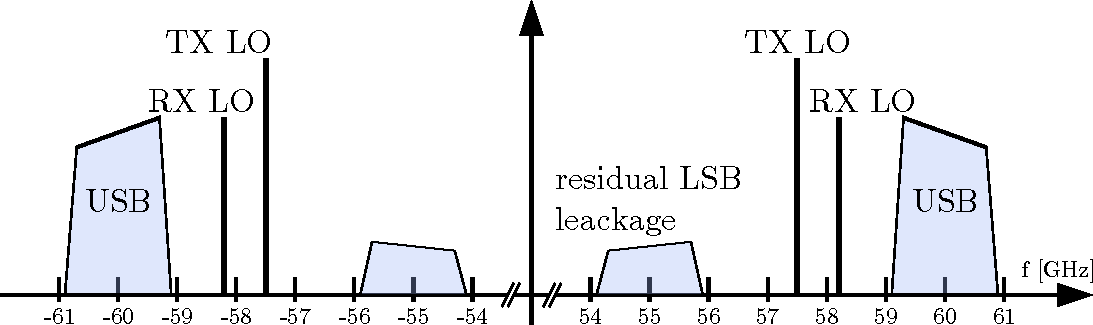
\includegraphics[width=0.8\textwidth]{figures/rx_2_freq_rf}
    \caption{\gls{RF}}
    \label{fig:rx_2_freq_rf}
  \end{subfigure}
  \vspace{4ex} \\
  \begin{subfigure}{\textwidth}
    \centering
    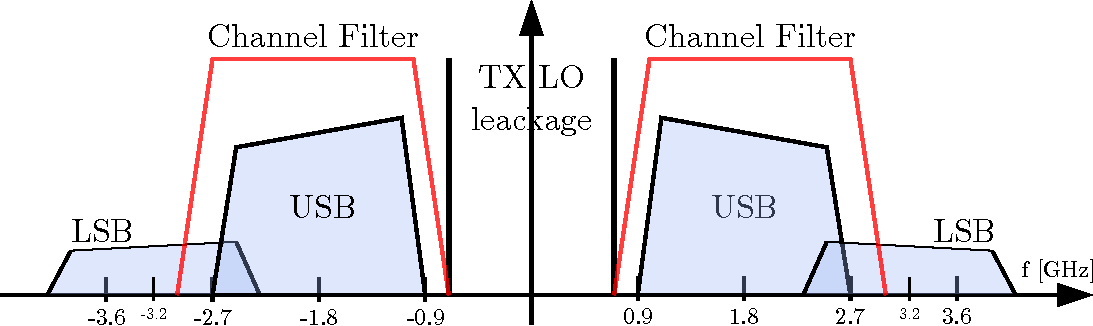
\includegraphics[width=0.8\textwidth]{figures/rx_2_freq_rx_if}
    \caption{\gls{RX} \gls{IF}}
    \label{fig:rx_2_freq_rx_if1}
  \end{subfigure}
  \vspace{4ex} \\
  \begin{subfigure}{\textwidth}
    \centering
    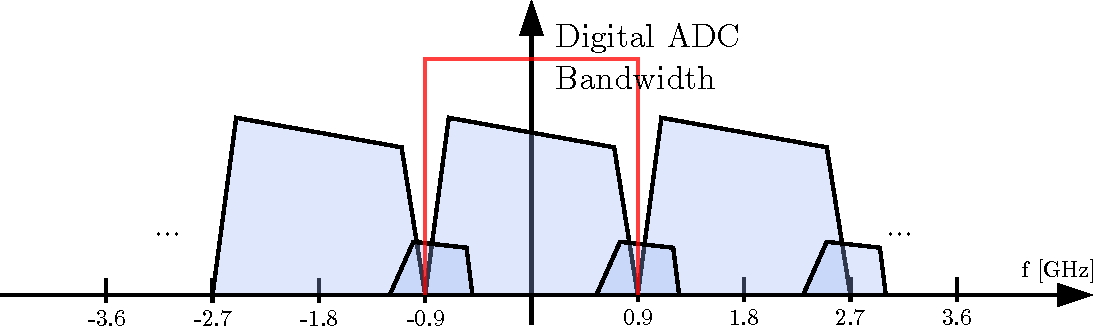
\includegraphics[width=0.8\textwidth]{figures/rx_2_freq_rx_adc}
    \caption{Sampled Signal}
    \label{fig:rx_2_freq_rx_if2}
  \end{subfigure}
  \caption{Quadrate Intermediate Frequency Sub-Nyquist Sampling Receiver
    in Frequency Domain}
  \label{fig:rx_2_freq}
\end{figure}

\section{Generation of Analytic Signal In Analog Domain}
\begin{itemize}
\item Explain how perfect analytic signal is created using hilbert transform
\item Explain how it is created using the sin/cos mixer
\item Explain error introduced in non perfect case
\end{itemize}
